\documentclass[compress]{beamer}
\usepackage{pgfpages}

\usepackage{amsmath}
\usepackage{amsthm}
\usepackage{amssymb, amstext, amsfonts, amscd, dsfont}

\usepackage{tikz}
\usepackage{tkz-euclide}

\usepackage{rotating}
\usepackage{wrapfig}

\newcommand{\RR}{\mathbb{R}}
\newcommand{\QQ}{\mathbb{Q}}
\newcommand{\NN}{\mathbb{N}}

% -- differentials --
\renewcommand{\d}{\partial\mspace{2mu}} % partial diff
%\renewcommand{\d}{\mathrm{d}\mspace{2mu}}
\newcommand{\td}{\,\mathrm{d}}  % total diff
\newcommand{\tdfrac}[2]{\frac{\td #1}{\td #2}}
\newcommand{\pdfrac}[2]{\frac{\d #1}{\d #2}}


\usetheme{Copenhagen}
\useoutertheme{split}

\setbeameroption{show notes}
%\setbeameroption{show notes on second screen=right}

\graphicspath{{images/}}

\setbeamertemplate{note page}{%
\insertnote%
}

%\setbeamertemplate{note page}{%
%\begin{wrapfigure}{r}{0.1\textwidth}%
%\rlap{\insertslideintonotes{0.25}}
%\end{wrapfigure}%
%\insertnote
%}

\title{Measure Theory and Probability}

\begin{document}
\begin{frame}
  \maketitle
  \note[item]{Lucas suggested to give a tutorial on measure theory.}
  \note[item]{I immediately agreed to to so, as I think measure theory is
              very important for quite some reasons.}
  \note[item]{First, it just explains what volume is and how you
              should think about it in order to avoid some problems,
              that you probably weren't even aware of}
  \note[item]{Then, it explains how you should think about
              integration and gives rise to a very powerful integral,
              much more powerfull and well-behaved than the Riemann
              integral that we usually are teached in school}
  \note[item]{Furthermore, it gives sense to these strange $\td x$-things
              in integration.}
  \note[item]{Also, it gives a solid foundation to the so called
              $\delta$-functions, that are loved a lot by physicists and
              hated by mathematicians, at least the way physicists use them}
  \note[item]{And last but not least, it gives a rich framework to build
              a unified probability theory on, that does not have to distinguish
              between a lot of different cases and that makes you aware of
              the subtle problems that can arise in probability theory, e.g.
              when dealing with conditional expectation values.}
\end{frame}


\begin{frame}
  \tableofcontents{}
  \note[item]{Mathematics of measure theory in parts quite technical.
    The proofs contain often formulas like ``an infinite union over an
    infinite intersection over an infinite union of some sets''.}
  \note[item]{Much more important when trying to understand measure theory: What
    is the problem measure theory is trying to solve?}  \note[item]{That is why
    I will start with some historical background and counterexamples that
    hopefully will give you an idea that there is a problem at all, that should
    be solved.}
\end{frame}
\section{Background}

\begin{frame}{Why Measure Theory}
  \begin{itemize}
  \item Ca. 1900: What is the volume of a subset of $\RR^n$?
  \end{itemize}
  \note[item]{Around 1900, mathematicians tried to come up with a
    universal definition of the notion of volume.}
  \note[item]{For quite a long time, they were able to work with their
    intuitive feeling for volume. But the development of set theory
    forced them to be more precise about their understanding of volume.}
  \note[item]{To show you that this is not as trivial as one might think,
    I want to show you some examples}
\end{frame}
\begin{frame}{What is volume?}
  \begin{minipage}{0.45\linewidth}
    \begin{center}
      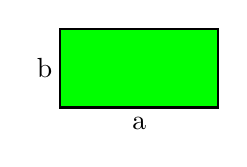
\begin{tikzpicture}[style=thick, fill=green]
        \draw[fill=green] (0,0) rectangle (2,1);
        \draw             (1.0, -0.2) node{a};
        \draw             (-0.2, 0.5) node{b};
      \end{tikzpicture}
    \end{center}
  \end{minipage}%
  \begin{minipage}{0.45\linewidth}
    $A = a \cdot b$
  \end{minipage}
  \note[item]<1->{This one is quite clear. The volume of a rectangle with sides
   $a$ and $b$ should be $a\cdot b$. More exactly: If we take the volume of
   the unit square to be one and want the volume to be multilinear, than we
   get this.}
  \pause
  \begin{minipage}{0.45\linewidth}
    \begin{center}
      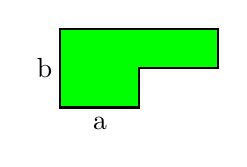
\begin{tikzpicture}[style=thick]
        \path[draw,fill=green] (0,0) -- (1,0) -- (1,0.5) -- (2, 0.5)
           -- (2,1) -- (0,1) -- cycle;
        \draw             (0.5, -0.2) node{a};
        \draw             (-0.2, 0.5) node{b};
      \end{tikzpicture}
    \end{center}
  \end{minipage}%
  \begin{minipage}{0.45\linewidth}
    $A = a \cdot b + \tfrac12 a \cdot b = \tfrac 32 \cdot a \cdot b$
  \end{minipage}
  \note[item]<2->{This example is not that more complicated. Intuitively we
    expect the volume to be additive. Thus we can divide this object into
    two rectangles}
  \pause

  \begin{minipage}{0.45\linewidth}
    \begin{center}
      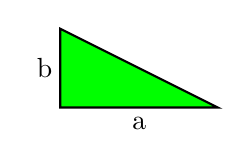
\begin{tikzpicture}[style=thick]
        \path[draw,fill=green] (0,0) -- (2,0) -- (0,1) -- cycle;
        \draw             (1.0, -0.2) node{a};
        \draw             (-0.2, 0.5) node{b};
      \end{tikzpicture}
    \end{center}
  \end{minipage}%
  \begin{minipage}{0.45\linewidth}
    $A = \tfrac12 a \cdot b$
  \end{minipage}
  \note[item]<3->{This equation becomes clear, if we divide a rectangle into two
    triangles which we then intuitively assume to have the same volume.}
\end{frame}

\begin{frame}{What is volume?}
  \note[item]<1->{Now what can we learn from the circle? Of course we all know
    that it's volume is $\pi r^2$, but how do we get this result? Obviously we
    cannot divide the circle into some rectangles. But maybe we can do something
    else.}
  \note[item]<2->{We can try to approximate the circle with shapes of known
    volume.  With a triangle, we can get only a very rough approximation of the
    circle.}
  \note[item]<3->{But with four triangles, we already get a much better
    approximation.}
  \note[item]<4->{Or with 10.}
  \note[item]<5->{With 16 triangles, we can hardly see the error of the
    approximation on this slide.}
  \note[item]<6->{In the limit, we expect to volume of the triangles to converge
    to the volume of the circle.}
  \begin{minipage}{0.45\linewidth}
  \begin{center}
    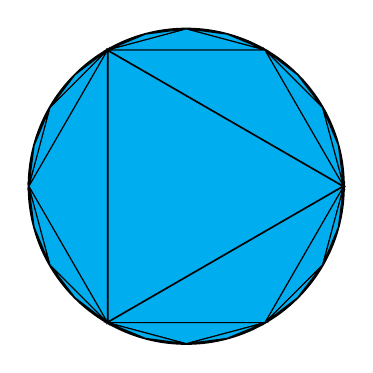
\begin{tikzpicture}[style=thick]
      \draw[fill=green] (0,0) circle (2);
      \pause
     % \draw             (1.0, -0.2) node{a};
      \path[draw,fill=cyan] (0:2)
      \foreach \x in {120,240}
        { -- (\x:2) } -- cycle;
      
      %\foreach \y in {0, 120, 240}
      %{
      %  \path[draw,fill=cyan] (\y:2)
      %  \foreach \x in {0,60,120}
      %   { -- (\x+\y:2) } -- cycle;
      %}
      \foreach \k in {3,6,12}
      { 
        \pause
        \foreach \x [evaluate=\x as \xx using (\x-1)*360/\k] in {1, ..., \k}
        { \path[draw,fill=cyan,style=thin] (\xx:2) 
          %\node{\x} at (\xx:2);
          \foreach \y [evaluate=\y as \yy using \xx+\y*360/\k/2] in {0,1,2}
          { -- (\yy:2) }
          -- cycle;
        }
      }
     \end{tikzpicture}
  \end{center}
  \end{minipage}%
  \begin{minipage}{0.45\linewidth}
    $\only<2-5>{A \geq A_1}
       \only<3-5>{+ 3A_2}
       \only<4-5>{+ 6 A_3}
       \only<5-5>{+ 12 A_4}$
    $\only<6>{A = A_1 + 3\sum_{n=0}^\infty 2^n A_{n+2}}$
  \end{minipage}
\end{frame}

%\setbeamercovered{transparent}
\begin{frame}{Why Measure Theory?}
  \note[item]<1->{Now let's sum up, what we have gained from our intuitive
    thinking on volume}
    \begin{definition}
      A volume is a function $\mathcal{P}(\RR^n) \to [0, \infty]$ such that
      \pause
      \begin{enumerate}[<+-| alert@+>]
      \item Positivity: $\mu_n(A) \geq 0$ for all $A \subset \RR^n$.
        \note[item]<2->{First, we want it to be positive (remember, we are
          talking about subsets. There is no way to distinguis $[a,b]$ from
          $[b,a]$ right now}
      \item Congruence: $\mu_n(A) = \mu_n(B)$ for all congruent $A$ and $B$.
        \note[item]<3->{Furthermore, we want it to be invariant under
          congruences.  That is, it should not change under rotation and
          mirroring. Otherwise the example with the triangle would not work}
      \item Norm: $\mu_n([0,1]^n) = 1$.
        \note[item]<4->{Then, we want one volume fixed: The one of the unit
          square.}
      \item $\sigma$-Additivity: $\mu_n(\bigcup_{i=1}^{\infty} A_i) =
        \sum_{i=1}^\infty \mu_n(A_i)$ for disjoint $A_i$.
        \note[item]<5->{And finally, we want it to be additive. But not only
          for finite unions, but even for countable unions. We need this
          property to be able to calculate the volume of the circle in
          the way I outlined.}
      \end{enumerate}
    \end{definition}
    %\pause
    \begin{lemma}<+->
      \begin{enumerate}
      \item $\mu_n(\{x\}) = 0$
      \item $\mu_n(A) \leq \mu_n(B)$ for $A \subseteq B$.
      \end{enumerate}
    \end{lemma}
    \note[item]<6->{From this properties, we already gain to important
      statements, that we don't have to demand in addition: Points have volume 0
      and the volume is monoton: If one shape contains another one, it has to
      have at least the same volume.}

\end{frame}

\begin{frame}{The vitali set}
  \note[item]<1>{Okay, now that we know how we would like our volume function
    to behave, we just have to find it. More precisely, mathematicians
    want to show that it exists and that it is unique. Till know,
    basically, there could be more than one volume functions with this
    property.}
  \note[item]<1>{This is what the mathematicians were trying to do at the
    beginning of the 20th century. But in 1904, the italian mathematician
    \textsc{Vitali} proved that such a volume function cannot exist at all.}
  \note[item]<1>{As his proof is quite easy, I am going to present it to you. It
    is crucial as without this phenomenon there would be no need for measure
    theory at all.}

  \pause

  Let $V$ be a set of representatives for the quotient group
  $\RR/\QQ$ from $[0,1]$, that is: For every $z \in \RR$, there is exactly one
  element of $z+\QQ$ in $V$ and this element lies within $[0,1]$.

  \note[item]<2>{We start with the quotient group $\RR/\QQ$. That is, we take
    $\RR$ and identify all numbers, that differ only by a rational number. Thus,
    for example, all rational numbers will be equal to 0 after the
    identification.}

  \note[item]<2>{Then from each class of identified numbers
    we take exactly one, that we furthermore demand to be from within the
    intervall $[0,1]$.}

  \note[item]<2>{This is the vitali set, for which we will show that it
    cannot have a well-defined volume.}

  \pause

  \note[item]<3->{First, we need two simple properties of the vitali set}

  \begin{lemma}
    \begin{enumerate}
    \item For $p\neq q$, $p,q\in\QQ$ we have $p+V \cap q+V = \emptyset$.
      \note[item]<3->{The first is, that arbitrary shifts of the vitali set by an
        rational offset are disjoint. That is simply by the very construction of
        the vitali set: If two of this shifts would not be disjoint, than this
        would say that two elements of the vitali set differ by a rational
        number. But then these two elements are in the same class of $\RR/\QQ$
        and hence the vitali set is allowed to contain at most one of
        them. [Whiteboard!]}
    \item Let $(p_n)_{n\in\NN}$ an enumeration of the rational numbers in
      $[-1,1]$ and $V_n=p_n + V$, then we have $[0,1] \subset
      \bigcup_{n=1}^{\infty} V_n \subset [-1, 2]$.

      \note[item]<3->{This one says that the union of all these shifts contain
        the unit interval and are contained in the interval $[-1,2]$.}
      \note[item]<3->{First the left inclusion: Let $x \in [0,1]$ and $\bar x$
        its class in $\RR/\QQ$. Then there is an $y \in \bar x$ with $y \in V$
        and $y-x = p_j \in \QQ$. As $x \in [0,1]$ and $y \in [0,1]$, $|x-y|\leq
        1$. Done. The right hand inclusion is trivial.}
    \end{enumerate}
  \end{lemma}
\end{frame}

\begin{frame}{The Vitali set}
  Let $\mu_1$ be a volume function on $\RR$.
 
  \note[item]{Now we can prove with the vitali set that we cannot have a
    well-defined volume on $\RR$. First we assume that is has a volume, that is,
    that there is a volume function on $\RR$.}  \pause


  Since $[0,1] \subset \bigcup_{n=1}^{\infty} V_n \subset [-1, 2]$, we have by
  monotony of the volume
  
  \[1 \leq \sum_{n=1}^\infty \mu_1(V_n) \leq 3,\]

  \note[item]<2->{As a volume has to be monotone (as I told you before), we get
    by $\sigma$-additivity that sum of the volumes of all the $V_n$ has to be
    between $1$ and $3$.}
  

  \pause
  but by congruence we have $\mu_1(V_n) = \mu_1(V)$ for all $n$, therefore

  \[1 \leq \sum_{n=1}^\infty \mu_1(V) \leq 3.\]

  \note[item]<3->{But as the $V_n$ are just shifts of the vitali set, they have
    to have all the same volume, thus we get that the countable infinite sum over
    the volume of $V$ has to be between $1$ and $3$.}

  \pause
  But if $\mu_1(V)=0$ then $\sum_{n=1}^\infty \mu_1(V)=0$ and if
  $\mu_1(V)>0$ then $\sum_{n=1}^\infty \mu_1(V) = \infty$. Therefore
  such a $\mu_1$ cannot exist.

  \note[item]<4->{But this is a contradiction: Either the volume of $V$ is $0$,
    then a countable sum of it is $0$ too, of course. Or it's volume is greater
    than zero. Then a countable sum over it is $\infty$. Therefore a volume
    function like desired cannot exist on $\RR$.}

\end{frame}

\begin{frame}{The Banach-Tarski Paradox}
  \note[item]{To resolve the problem shown by the Vitali set, several ways were
    suggested. One was to give up the $\sigma$-additivity. However, this is an
    important property that is crucial for a lot of important theorems. And
    furthermore, Banach and Tarski were able to show that even with usual
    additivity, in dimension greater or equal 3 one gets problems.}
  \pause
  \begin{theorem}[Banach-Tarski]
    Given a solid sphere in 3-dimensional space, there exists a decomposition of
    the sphere into five disjoint subsets (i.\,e., non-overlapping pieces),
    which can be put back together in a different way (only using isometries) to
    yield two identical copies of the original sphere.
  \end{theorem}
  \pause
  \includegraphics[width=\linewidth]{Banach-Tarski_Paradox-Illustration.png}
  \rotatebox{90}{\tiny{Source: Wikipedia}}
\end{frame}

\begin{frame}{The Banach-Tarski Paradox}
  \begin{itemize}
  \item Proof is a little bit technical, but perfectly understandable with very
    little mathematical background \note[item]{For those interested in it: There
      is a very nice book by Leonard Wapner, \textit{Aus 1 mach 2}, that tells
      the story behind this theorem and also give a version of the proof that is
      perfectly understandable even with no mathematical background. Also there
      is a good article in the \textit{Mathematical intelligencer}, that gives
      an proof that is quite easy to understand.}
  \item Ingrediences
    \begin{itemize}
    \item Shifting to infinity (``Trick of Hilbert's Hotel'')
    \item Paradoxial decomposition of a group generated by two rotations $f$ and $g$ into $I$, $J$, $K$, i.\,e., such that $fI = J \cup K$, $gI = J$, $g^2I = K$
    \item Axiom of choice
    \end{itemize}
  \end{itemize}
\end{frame}

\section{Measure Theory}

\begin{frame}{So far}
  \begin{itemize}
  \item We cannot have volume function for all subsets of $\RR^n$.
  \item We do not want to give up any of the postulated properties
    of a volume function.
  \item Solution: Define it only on a specific set of subsets.
  \item This subset has to have certain properties to enable us
    to do the usual calculations for volumes
  \end{itemize}
\end{frame}

\begin{frame}{$\sigma$-algebras}
  \begin{definition}[$\sigma$-algebra]
    Let $\Omega$ be a set. Then a set $\mathcal{A} \subset \mathcal{P}(\Omega)$
    is called $\sigma$-algebra, if it satisfies the following properties:
    \begin{enumerate}
    \item $\Omega \in \mathcal{A}$
    \item Closed under complements: $X \in \mathcal{A} \Rightarrow
      \Omega\setminus X \in \mathcal{A}$
    \item Closed under countable unions: If $X_n \in \mathcal{A}$ for all $n$,
      then $\bigcup_{n=1}^\infty X_n \in \mathcal{A}$.
    \end{enumerate}
  \end{definition}
  \note[item]{The $\sigma$-algebra encaspulates all the properties that we want
    the set of ``usable'' sets to fullfill}
  \pause
  \begin{example}
    \begin{enumerate}
    \item Borel $\sigma$-algebra $\mathcal{B}$ generated by all intervals
      $[a,b]$ on $\RR$.
    \item The set of all subsets $\mathcal{P}(X)$ for some set $X$ (suitable
      usually only for countable sets).
    \end{enumerate}
  \end{example}
  \note[item]<2->{The Borel algebra is maybe the most important example, as it
    is the set of sets for that a ``volume'' can be defined in $\RR^d$. It will
    also play an important role in probability theory on $\RR^d$. It
    basically consists of all sets where the volume is obviously defined,
    i.e. intervals. And furthermore, it contains all sets that we need
    to get a proper $\sigma$-algebra out of this. This is actually the
    definition of the Borel algebra: It is the smallest $\sigma$-algebra,
    that contains all intervals $[a,b]$.}
  \note[item]<2->{If the base set is only countable, all the presented
    pathologies do not work and we can use all subsets.}
\end{frame}

\begin{frame}{Measures}
  \begin{definition}[measure]
    Let $\Omega$ be a set and $\mathcal{A}$ be a $\sigma$-algebra on
    $\Omega$. Then a function $\mu: \mathcal{A} \to [0, \infty]$ is called a
    measure, if:
    \begin{enumerate}
    \item $\mu(\emptyset) = 0$
    \item $\sigma$-additivity: If $X_n \in \mathcal{A}$ are pairwise disjoint,
      then $\mu(\bigcup_n X_n) = \sum_n \mu(X_n)$.
    \end{enumerate}
  \end{definition}
  \note[item]{Now, that we have resolved the problems with pathological sets by
    excluding them in a well-defined manner, no problems rise when defining such
    a thing as a volume function. We do it in a more general way (no
    normalization, no invariance under congruence) as that is not needed for the
    theory and call it \textit{measure} instead of volume function: The measure
    is the base object for things like volume functions or later also
    probabilities}
  \begin{example}
    \begin{enumerate}[<+->]
    \item Lebesgue measure $\mu$ on $\RR$ with $\mathcal{B}$: The extension of
      $\mu([a,b])=b-a$ to $\mathcal{B}$ (it is all but trivial that it exists
      and is well-defined).
    \item Counting measure on $\NN$ with $\mathcal{P}(\NN)$: $\mu(X) = \#X$.
    \item Delta-measure $\delta$ on $\RR$: $\delta(X)=1$ if and only if $0 \in
      X$, else 0.
    \end{enumerate}
  \end{example}
  \note[item]<2->{The most important measure is the Lebesgue measure, which
    encapsulates the volume on $\RR$ resp. $\RR^d$.}
  \note[item]<3->{Also of important is the counting measure, which measures a
    set by just counting it.}
  \note[item]<4->{The delta measure is basically what the delta functions become
    in measure theory: It gives a set measure 1 if and only if it contains a
    specific point, e.g. zero. Therefore it measures wheter a set contains
    this point.}
\end{frame}

\begin{frame}{Integration theory}
  \begin{definition}[measurable function]
    Let $\Omega_1$, $\Omega_2$ be sets with $\sigma$-algebras $\mathcal{A}_1$,
    $\mathcal{A}_2$. Then a function $f: \Omega_1 \to \Omega_2$ is called
    \textit{measurable}, if $f^{-1}(X) \in \mathcal{A}_1$ for all $X \in
    \mathcal{A}_2$.
  \end{definition}
  \begin{itemize}
  \item Important for integration: The measure integral divides
    horizontally, not vertically.
  \item Important for probability theory: Random variables will be
    measurable functions
  \end{itemize}
  \note[item]{Urbild=Fiber: Fibers of measurable sets are measurable}
\end{frame}

\begin{frame}{Integration theory}
  \note[item]{Now we have all the definitions to define the measure
     integral. You might wonder, why I care to define a new integral here,
     you are probably just interested in probability theory. But
     probability theory relies heavily on the measure integral, as you
     will see later. Therefore I have to show it to you.}
  Let $f: \Omega \to \RR$ be measurable and elementary: It takes only
  finitely many values $\alpha_i$ on the disjoint measurable sets
  $A_i$. Then we define
  \[
    \int_{\Omega} f\td \mu := \sum_{i=1}^n \alpha_i\mu(A_i)
  \]

  \begin{center}
    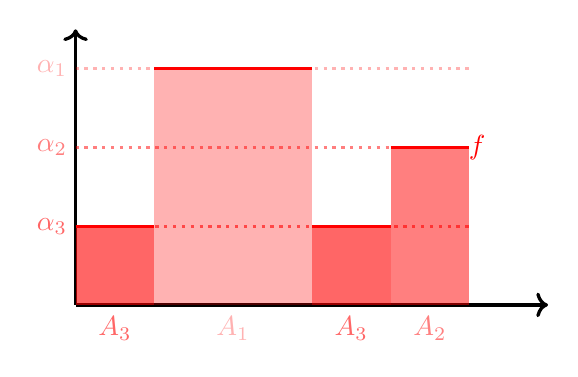
\begin{tikzpicture}[style=very thick]
      \draw[->] (0,0) -- (6,0);
      \draw[->] (0,0) -- (0,3.5);
      \draw[red] (0,1) -- (1,1)
                 (1,3) -- (3,3)
                 (3,1) -- (4,1)
                 (4,2) -- (5,2);
      \draw[red] (5.1,2) node{$f$};
      %\pause
      \visible<2->{
      \fill[fill=red,opacity=0.3] (1,0) rectangle (3,3);
      \draw[red,opacity=0.3] (2,-0.3) node{$A_1$};
      \draw[red,opacity=0.3] (-0.3,3) node{$\alpha_1$};
      \draw[dotted,red,opacity=0.3] (0,3) -- (5,3);}
      %\pause

      \visible<3->{
      \fill[fill=red,opacity=0.5] (4,0) rectangle (5,2);
      \draw[red,opacity=0.5] (4.5,-0.3) node{$A_2$};
      \draw[red,opacity=0.5] (-0.3,2) node{$\alpha_2$};
      \draw[dotted,red,opacity=0.5] (0,2) -- (5,2);}
      %\pause
      \visible<4->{
      \fill[fill=red,opacity=0.6] (0,0) rectangle (1,1);
      \fill[fill=red,opacity=0.6] (3,0) rectangle (4,1);
      \draw[red,opacity=0.6] (0.5,-0.3) node{$A_3$};
      \draw[red,opacity=0.6] (3.5,-0.3) node{$A_3$};
      \draw[red,opacity=0.6] (-0.3,1) node{$\alpha_3$};
      \draw[dotted,red,opacity=0.6] (0,1) -- (5,1);}
    \end{tikzpicture}
  \end{center}
\end{frame}

\begin{frame}{Integration theory}
  By a limit process (formal completion), the integral is extended to a space
  $L_1$ of integrable ``functions''.
  \begin{center}
    \includegraphics[width=0.7\linewidth]{Riemannvslebesgue.png}
    \rotatebox{90}{\tiny Wikipedia}
  \end{center}
\end{frame}

\begin{frame}{Integration theory}
  \begin{itemize}
  \item More integrable functions: $\int_\RR \chi_\QQ \td x= 0$.
  \item Much better convergence properties, e.\,g. dominated convergence: $f_n
    \in L_1$, $f_n \to f$ pointwise and $|f_n|\leq g$ for some $g \in L_1$, then
    $f \in L_1$ and $\int f = \lim \int f_n$ (For comparison: The Riemann
    integral needs uniform convergence for this property).
  \item Notation: If the integrated variable is needed, we write
   \[
     \int_X f(x) \td \mu(x) := \int_X f\td \mu
   \]
 \item Also generalization of finite and countable sums: With the counting
   measure $c$:
    \[ \sum_{i=0}^\infty \alpha_i = \int_\NN \alpha(i) \td c(i) \]
  \end{itemize}
  \note[item]{Although the meaning of the last point might not be that obvious,
    it is crucial especially for probability theory, as it says that we can
    prove theorems for discrete, continuous and other distributions at the same
    time.}
\end{frame}

% \begin{frame}{Radon-Nikodým theorem}
%   \begin{theorem}[Radon-Nikodým]
%     Let $(X, \Sigma)$ be a measurable space, $\nu$ and $\mu$ $\sigma$-finite
%     measures on $X$. If $\nu$ is absolutely continuous with respect to $\mu$,
%     i.\,e., $\mu(A) = 0 \Rightarrow \nu(A) = 0$, then there is a measurable
%     function $f: X \to [0, \infty)$, such that
%     \[
%       \nu(A) = \int_A f \td \mu
%     \]
%     The function $f$ is called \textit{Radon-Nikodym derivative} of $\nu$ with
%     respect to $\mu$ and often written as $f = \frac{\td \nu}{\td \mu}$.
%   \end{theorem}
%   \note[item]{This theorem is crucial for probability theory, as it tells us,
%     when a probability distribution has a density function like we are used to
%     it. Also it is necessary to show, that conditional expectation values exist.}
% \end{frame}

\section{Probability Theory}

\begin{frame}{Probability theory}
  \begin{definition}[Probability space]
    A \textit{probability space} is a measure space $(\Omega, \mathcal{F}, P)$,
    such that $P[\Omega]=1$.  The set $\Omega$ is called set of
    \textit{outcomes}, the elements of the $\sigma$-algebra $\mathcal{F}$ are
    called \textit{events} and the measure $P$ is called \textit{probability
      measure}
  \end{definition}
  \pause
  \begin{example}[Fair dice roll]
    $\Omega=\{1,2,3,4,5,6\}$, $\mathcal{F} = \mathcal{P}(\Omega)$, $P[A] =
    \frac16\cdot \#A$. $A_{\text{odd}}=\{1,3,5\}$.
  \end{example}

  \begin{example}[Uniform on $I$]
    $\Omega=\RR$, $\mathcal{F} = \mathcal{B}(\RR)$, $P[A] = \int_A \chi_I(x)\td
    x$.
  \end{example}
\end{frame}

\begin{frame}
  Why this complicated?
  \begin{itemize}
  \item It is not enough to specify $P[\{\omega\}]$ only for outcomes: If
    $\Omega$ is infinite, then one might have $P[\{omega\}]=0$ for all $\omega$
    (e.g. uniform distribution).
  \item It is in general not possible to specify $P[A]$ for all $A \subset
    \Omega$: We can construct vitali sets also for probability theory, e.g. for
    $\Omega = \{0,1\}^\NN$, i.\,e. countably many coin throws.
  \item ``But for continuous distributions, we have the pdf!'': Theory becomes
    unnecessary complicated, if we have to distinguish all the time between
    continuous and discrete distributions. Later: It is even more general.
  \end{itemize}
\end{frame}

\begin{frame}{Probability measures and density functions}
  \begin{itemize}
  \item Obvious: For a pdf $p(x)$ on $\RR^d$, we get a probability measure by
    $P(A) = \int_A p(x)\td x$
  \item When does the reverse hold?
  \pause
  \begin{theorem}[Radon-Nikodým]
    Let $(X, \Sigma)$ be a measurable space, $\nu$ and $\mu$ $\sigma$-finite
    measures on $X$. If $\nu$ is absolutely continuous with respect to $\mu$,
    i.\,e., $\mu(A) = 0 \Rightarrow \nu(A) = 0$, then there is a measurable
    function $f: X \to [0, \infty)$, such that
    \[
      \nu(A) = \int_A f \td \mu
    \]
    The function $f$ is called \textit{Radon-Nikodym derivative} of $\nu$ with
    respect to $\mu$ and often written as $f = \frac{\td \nu}{\td \mu}$.
  \end{theorem}
  \end{itemize}
  \note[item]<2->{This theorem is crucial for probability theory, as it tells us,
    when a probability distribution has a density function like we are used to
    it. Also it is necessary to show, that conditional expectation values exist.}

\end{frame}

\begin{frame}{Probability measures and density functions}
  \begin{itemize}
  \item Allows us to define the usual pdf $p(x)$ for Probability measures with
    $P[X]=0$ for all $X \in \mathcal{B}(\RR^d)$ with respect to the Lebesgue
    measure.
  \item Allows us to definie the usual pdf $p(x)$ for discrete Probability
    measures with respect to the counting measure on countable sets.
  \end{itemize}
\end{frame}

\begin{frame}{Beyond discrete and continuous distributions}
  \begin{example}[Sparse variable]
    Let $[a,b]\subseteq [0,1]$
    \[
      P[[a,b]]=
      \begin{cases}
        \tfrac12(b-a) & \tfrac12 \notin [a,b]\\
        \tfrac12(b-a) + \tfrac12 & \frac12 \in [a,b]
      \end{cases}
    \]
    This is the measure of a probability space where we get the value $0$ with
    probability $\tfrac12$ and otherwise a uniform distribution on $[0,1]$,
    i.\,e. a mixture of a discrete and a continuous distribution.
  \end{example}
\end{frame}

\begin{frame}{Beyond discrete and continuous distributions}
  %The cantor set: Iterated cutting out the middle of an interval.
  \[\text{The cantorset } C = \bigcap_{i=0}^\infty \bigcup_{j=0}^{2^i} I_{i,j}\]
  \begin{center}
    \begin{tikzpicture}
      \input{cantor_test}
    \end{tikzpicture}
  \end{center}
  \pause
  \begin{example}[Cantor distribution]
    On $\RR$ we define a probability measure by $P[I_{i,j}] = 2^{-i}$. This is
    not a discrete measure (every point has probability zero), nor is it a
    continuous distribution (it has no density) nor a mixture of this two.
  \end{example}
  \note[item]<2->{The cantor distribution is not discrete, as every point as
    probability zero. It cannot have a density, since the cantor set is a zero
    set with respect to the Lebesque measure. It cannot be a mixture for the
    same reason as in the discrete case.}
\end{frame}

\begin{frame}[Random variables]
  \begin{definition}[Random variable]
    Let $(\Omega, \mathcal{F}, P)$ be a probability space. A \textit{random
      variable} is a measurable function $X: \Omega \to \Omega_2$ for some
    measurable space (i.\,e., a space with a $\sigma$-algebra). Usually
    $\Omega_2=\RR^d$ with the Borel algebra.
  \end{definition}
  \note[item]{The function has to be measureable: This tells us that $P[X\in A]$
    for all $A$ in the $\sigma$-algebra on $\Omega_2$. In other words: A random
    variable induces a probability measure $P_X$ on $\Omega_2$.}

  \begin{example}[Double dice roll]
    $\Omega=\{1, \dots, 6\}^2$. Then $f_{\text{sum}}((\omega_1, \omega_2)) =
    \omega_1+ \omega_2$ is a random variable.
  \end{example}
\end{frame}

\begin{frame}[Random variables]
  \begin{definition}[expectation value]
    Let $X$ be a random variable on a probability space $(\Omega, \mathcal{F},
    P)$. Then the \textit{expection value} is given by
    \[
      E[X] = \int_{\Omega} X(\omega) \td P(\omega)
    \]
    if this integral exists. In the case of discrete or continous distributions,
    this specializes to the usual definitions.
  \end{definition}
\end{frame}

\begin{frame}{Examples}
  \begin{itemize}
  \item Entropy: $\sum_x p(x)\log p(x)$, $\int p(x)\log(p(x))\td x$ becomes
   \[
     \int_{\Omega} \log(p(\omega))\td P(\omega)
   \]
 \item Kullback-Leibler-Divergence: $\sum_x p(x) \log\frac{p(x)}{q(x)}$, $\int
   p(x) \log\left(\frac{p(x)}{q(x)}\right) \td x$ becomes
   \[
     \int_{\Omega} \log\left(\frac{p(\omega)}{q(\omega)}\right) \td P(\omega)
   \]
  \end{itemize}
\end{frame}

\begin{frame}{Examples}
  Mixture of gaussians: 
\end{frame}

\begin{frame}{TODO}
  Applications: Sparse coding: Mixture of discrete and continuous distribution.

  Fubini: Integralvertauschungen sind gefährlich

  Radon-Nikodym

  mixture of discret+continuierlich
\end{frame}

\end{document}
